\documentclass[a4paper,10pt]{article}

\usepackage{fancyhdr} % clears the header and footer setting
\usepackage{graphicx} 
\usepackage{geometry}
\geometry{a4paper, left=2cm, right=2cm, top=1.5cm, bottom=3cm }
\usepackage{caption}
\usepackage{subcaption}
\usepackage{hyperref}
\usepackage{natbib}
\usepackage{amsmath}


\usepackage{etoolbox,fancyhdr,xcolor}
\newcommand{\headrulecolor}[1]{\patchcmd{\headrule}{\hrule}{\color{#1}\hrule}{}{}}
\newcommand{\footrulecolor}[1]{\patchcmd{\footrule}{\hrule}{\color{#1}\hrule}{}{}}
\renewcommand{\headrulewidth}{1pt}
\headrulecolor{black!100}%
\renewcommand{\footrulewidth}{1pt}
\footrulecolor{red!100}%

\fancyhf{}
\fancyhead[R]{
\includegraphics[width=0.25\textwidth]{nmims.png}}

\fancyfoot[C]{Nilkamal School of Mathematics, Applied Statistics & Analytics}
\fancyfoot[R]{\thepage}

\setlength{\headheight}{15mm}
\pagestyle{fancy} %This command sets the page style to fancy, applying the header and footer configurations defined above to the document pages.

\bibliographystyle{apacite}

\usepackage{times}
\begin{document}

\noindent 
\begin{center}
\textbf{{\Large Movie Recommendation System Using Collaborative Filtering and Content-Based Filtering}} \\
\end{center}

\noindent 
\begin{center}
\textbf{ Zaamena Shamji, Anushka Jain, Neha Maheshwari, Nitya Verma, Aditee Gupta } 
\end{center}\\[-0.5cm]

\begin{center}
\textit{Narsee Monjee Institute Of Management Studies, Mumbai}\\
\end{center}


\noindent 
\begin{center}
    \subsection*{ABSTRACT}
    This project revolves around building a movie recommender system based on conventional techniques like Content-based and drawing up a comparison between them to better understand the implementation of the same by a large number of tech companies. The primary purpose of the project is to build a movie recommender system for new users of an emerging brand in the market.

\end{center}

\noindent 
\textbf{KEYWORDS:} \textit{Collaborative Filtering},\textit{Content-Based Filtering},\textit{Singular Value Decomposition}


\section{INTRODUCTION}

The research objective is to develop and understand the workings and usage of a movie recommendation system. A recommendation system refers to a platform or an engine that provides suggestions for items. The purpose of the recommendation system is to suggest items or products of interest to the users. It studies the relationship between the items and the users to give specific recommendations.

With the increasing growth of content on over-the-top platforms, users often face information load and get overwhelmed. This makes it difficult for the users to choose content that is relevant to their preferences and a one-size-fits-all approach may not be effective. A recommendation system aids diverse users in getting recommendations according to individual tastes and preferences. It helps users narrow down the wide and confusing horizon of options and saves them the time and effort to go through each and every product. This not only helps users get a personalized experience but also assists them in discovering new content that would have been otherwise overlooked due to popular content.

Highly regarded companies like Amazon, Netflix and Spotify use these methods to enhance their customer experience. Their recommendation system utilizes the user's interaction history, their preferences and their similarity with other users to provide recommendations.

For movie recommendations, the project utilizes two types of techniques to provide personalized and relevant suggestions to the users:

\begin{enumerate}
    \item Content-Based Filtering: This method utilizes the past behaviour of the user, to suggest products that are similar to the previously used product of the user. Attributes such as genre, director, actors and generated tags or keywords are analyzed to identify similarities between movies.

    \item Collaborative Filtering: As for collaboration, instead of finding similarities between the items based on the user behaviour, it finds similarities between multiple users and cross-suggests their products to each other. This technique further bisects into two approaches, namely, item-based filtering and user-based filtering.
    \begin{itemize}
        \item Item-based Collaborative Filtering: This focuses on the similarities between the items or the products. Any items sharing similar features are cross-recommended to users who like either of the products.

        \item Model-based Collaborative Filtering:
        This method helps to predict similar movies according to users past interactions as well as other users who are similar to them. This technique requires matrix factorization, which decomposes the user-item interactions to represent latent features.

    \end{itemize}
    
\end{enumerate}

By employing these techniques, the research aims to improve user satisfaction and engagement. This will help the platform to increase viewership and potentially increase revenue.

\section{LITERATURE REVIEW}

\section{DATA}

\subsection{Data Collection}


A secondary research was conducted for this project.  \textbf{Netflix Prize Dataset} (\cite{netflix_prize_data})  and \textbf{Netflix Titles} (\cite{soeiro_n.d.}) datasets were taken into account for building the recommendation system. Both the datasets are available on Kaggle.com \cite{kaggle}. The "Netflix prize" dataset is the official dataset published by Netflix for an open competition. 

The "Netflix Titles" dataset is an entirely different dataset containing detailed information about each movie.

\subsection{Data Structure}

\textbf{\textit{Netflix Prize Data}} comprises of two text file. The first dataset contains information of the ratings given by the customer to each movie. Table \ref{Data_1} shows the structure of the dataset wherein 

\begin{itemize}
  \item MovieIDs: The unique ID assigned to each movie. It ranges from 1 to 17023 sequentially.
  \item CustomerIDs: The unique ID assigned to each customer. It range from 1 to 2649429, with gaps.
  \item Ratings: Ratings given by each customer. They are on a five-star (integral) scale from 1 to 5.
  \item Dates have the format YYYY-MM-DD.
\end{itemize}
The table shows the ratings given by three different customers to movie Id 1 on the given dates. 






\begin{table}
    \center 
    
    \begin{tabular}{|c|c|c|c|} \hline 
         Customer ID&  Movie ID&  Rating& Date\\ \hline 
         1488844&  1&  3& 2005-09-06
\\ \hline 
         822109&  1&  5& 2005-05-13
\\ \hline 
         885013&  1&  4& 2005-10-19
\\ \hline
    \end{tabular}
    \caption{Customer Rating}   
    \label{Data_1} 
\end{table}

The second dataset contains the titles of the movies corresponding to their respective movie IDs. Table \ref{Movie_titles} shows the structure of the \textit{\textbf{movie titles}} dataset. 

\begin{table}
    \centering
    \begin{tabular}{|c|c|l|} \hline 
         Movie ID& Year Of Release&Title\\ \hline 
         1& 2004&Dinosaur Planet\\ \hline 
         48&  2001&Justice League\\ \hline 
         198
&  1997&Gupt\\ \hline
    \end{tabular}
    \caption{Movie Titles Dataset}
    \label{Movie_titles}
\end{table}

\vspace{10pt}
Figure \ref{netflix titles} shows \textbf{\textit{Netflix Titles}} dataset which contains  information of the movies/Tv shows on Netflix. The dataset contains \textbf{8807} movies in total. The features in the dataset are as follows 
\begin{itemize}
    \item \textbf{Show ID}: Unique ID for every Movie / Tv Show. 
    \item \textbf{Type}:Identifies whether it is A Movie or TV Show 
    \item \textbf{Title} :Title of the Movie / Tv Show 
    \item \textbf{Director}: Director of the Movie
    \item \textbf{Cast}: Actors involved in the movie / show
    \item \textbf{Country}: Country where the movie / show was produced
    \item \textbf{Date} Added: Date it was added on Netflix
    \item \textbf{Release} \textbf{Year}: Actual Release year of the move / show
    \item \textbf{Rating}: TV Rating of the movie / show
    \item \textbf{Duration}:Total Duration - in minutes or number of seasons
    \item \textbf{Listed In}: Genre of the movie/ Show
    \item \textbf{Description}:The summary description 
\end{itemize}
\begin{figure}
    \centering
    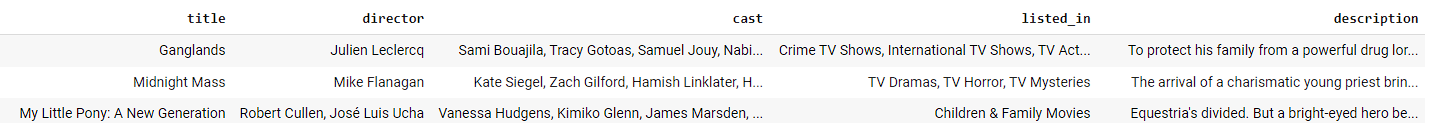
\includegraphics[width=1\linewidth]{figures/netflix_title.png}
    \caption{Netflix Titles Dataset}
    \label{netflix titles}
\end{figure}





\section{Methodology}

\subsection{Data Cleaning}

All the datasets were checked for missing and duplicate values. 
The unnecessary columns like \textit{Date}, \textit{Year Of Release}, \textit{Duration}, etc were deleted. The missing values were either replaced by an empty string, in the case of attributes, or by a zero in the case of numerical columns.  


\subsection{Data Preprocessing}

\subsubsection{Collaborative Filtering}
\textit{\textbf{Netflix Prize dataset}} was used for item-based collaborative filtering. 
\begin{itemize}
    \item \textbf{Merging}: The two datasets (\ref{Data_1} and \ref{Movie_titles}) within the Netflix prize dataset were merged based on the common attribute \textit{MovieID}. The new dataset is given in the figure \ref{Movie_merge}
\end{itemize}

\begin{figure}[ht]
\centering
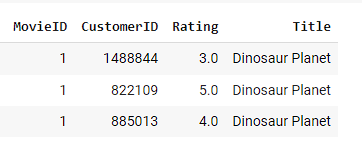
\includegraphics[height=4cm]{figures/movie_data.png}
\caption{Merged Data}
\label{Movie_merge}
\end{figure}


\begin{itemize}
    \item \textbf{Outliers}: The count of ratings given to each movie was calculated. The average count of ratings turned out to be around 26. The outliers were removed by the given formula 
\end{itemize}

\begin{enumerate}
  \item Interquartile Range (IQR):
    \[ \text{IQR} = Q3 - Q1 \]

  \item Upper Limit for Outliers:
    \[ \text{Upper Bound} = Q3 + 1.5 \times \text{IQR} \]
\end{enumerate}

\subsubsection{Content Based Filtering}:

\textbf{\textit{Netflix Titles}} \ref{netflix titles} was used to for content based filtering

\begin{itemize}
    \item \textbf{Stop word removal}: Stopwords are those words which do not add any meaning to the data and are used only to make sense of the information. Words like \textit{a}, \textit{an}, \textit{the}, etc are considered as stopwords. Such words can be removed from the data to increase computational efficiency. 
\end{itemize}


\begin{itemize}
    \item \textbf{Vectorization}: For algorithms to understand textual data, vectorization is used to convert any such data into a numerical value. Vectorization is a natural language processing technique. There are many different methods to perform this process like Bag of Words, TF-IDF, and Word2Vec.We have used Bag of Words to vectorized our data
\end{itemize}

\begin{itemize}
    \item \textbf{Stop word removal}: Stopwords are those words which do not add any meaning to the data and are used only to make sense of the information. Words like \textit{a}, \textit{an}, \textit{the}, etc are considered as stopwords. Such words can be removed from the data so as to increase computational efficiency
\end{itemize}

\begin{itemize}
    \item \textbf{Stemming}: Stemming refers to the process of conversion of words to their base/root form. For example, learn, learning, learned etc have the same meaning, hence they can be converted into their root form that is \textit{learn}. Stemming also helps in increasing the accuracy and reduces the duplication. 
\end{itemize}



Figure \ref{sigmoid} shows an S-shaped graph of a sigmoid function. 


\begin{figure}[ht]
\centering
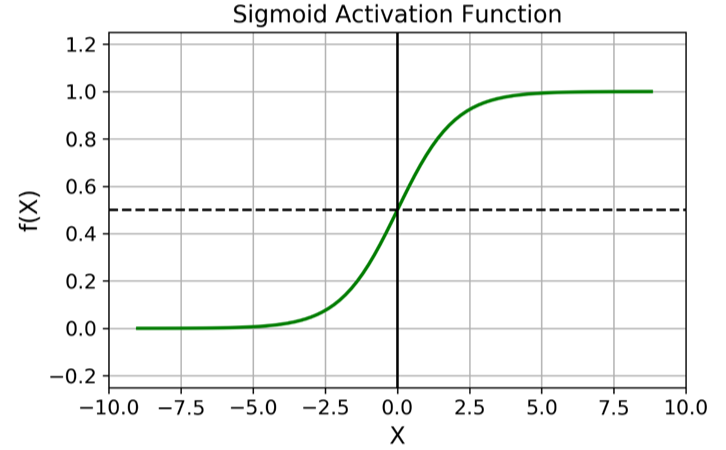
\includegraphics[height=6.6cm]{figures/sigmoid.png}
\caption{Sigmoid Function}
\label{sigmoid}
\end{figure}

(\ref{sigmoid_eq}) shows the equation of a sigmoid function where $x$ is any real-valued number which needs to be converted into a number between 0 and 1

\begin{equation}
f(x) = \frac{1}{1 + e^{-x}}
\label{sigmoid_eq}
\end{equation}

\subsection{Data}
\subsubsection{Data Collection}

The data is stimulated using Python and AI tools. An overview of the variables considered in the data was taken by going through different research papers and articles. 

\subsubsection{Data Summary}
The sample encompasses the purchase decisions made by customers regarding various products, which may or may not feature green packaging.The dataset has 330 customers and their information. 
The data consists of the following variables
\begin{itemize}

    \item Income 
    \item Age 
    \item Gender 
    \item Price of the product
    \item Type of product
    \item Green packaging (Yes/No)
    \item Purchase Decision (Yes/No)
\end{itemize}

Whether the customer purchased the product or not is the dependent variable and the rest are independent variables. 

\begin{table}[h]
\centering
\caption{Summary Statistics}
\begin{tabular}{|l|l|l|l|l|l|l|}
\hline
\textbf{Index} & \textbf{Age} & \textbf{Income} & \textbf{Gender} & \textbf{Price} & \textbf{Green Pack} & \textbf{Purchase} \\
\hline
Count & 330 & 330 & 330 & 330 & 330 & 330 \\
\hline
Mean & 40.188 & 79093.939 & 0.500 & 2305.558 & 0.545 & 0.661 \\
\hline
Std & 10.561 & 31987.012 & 0.501 & 1251.297 & 0.499 & 0.474 \\
\hline
Min & 20 & 25000 & 0 & 300 & 0 & 0 \\
\hline
25\% & 31 & 52250 & 0 & 1200 & 0 & 0 \\
\hline
50\% & 40 & 78000 & 0.5 & 2050 & 1 & 1 \\
\hline
75\% & 49 & 98000 & 1 & 3206.75 & 1 & 1 \\
\hline
Max & 60 & 160000 & 1 & 4932 & 1 & 1 \\
\hline
\label{summary_statistic}
\end{tabular}
\end{table}

Table \ref{summary_statistic} shows the summary statistic of all the variables. The average price is  2305.558 and the mean income of the customers is 79093.939. The lowest income is 25000 and the maximum income is 160000



\begin{table}[h]
\centering
\caption{Correlation Matrix}
\begin{tabular}{|l|l|l|l|l|l|l|}
\hline
 & \textbf{Age} & \textbf{Income} & \textbf{Gender} & \textbf{Price} & \textbf{Green Pack} & \textbf{Purchase} \\
\hline
\textbf{Age} & 1.00 & 0.87 & -0.07 & 0.69 & -0.17 & 0.33 \\
\hline
\textbf{Income} & 0.87 & 1.00 & -0.03 & 0.81 & -0.14 & 0.41 \\
\hline
\textbf{Gender} & -0.07 & -0.03 & 1.00 & -0.04 & -0.16 & -0.06 \\
\hline
\textbf{Price} & 0.69 & 0.81 & -0.04 & 1.00 & -0.21 & 0.35 \\
\hline
\textbf{Green Pack} & -0.17 & -0.14 & -0.16 & -0.21 & 1.00 & -0.06 \\
\hline
\textbf{Purchase} & 0.33 & 0.41 & -0.06 & 0.35 & -0.06 & 1.00 \\
\hline
\label{Correlation_matrix}
\end{tabular}
\end{table}

Table \ref{Correlation_matrix} shows the correlation among the numerical variables. It is evident from the table that the \textit{Income} of the customers and the \textit{Purchase decision} of the customers are positively correlated. 
It is also apparent that there is a negative correlation between the \textit{age} of the customers and the decision to \textit{buy} the product



\subsection{Case Analysis}


\begin{figure}[ht]
\centering
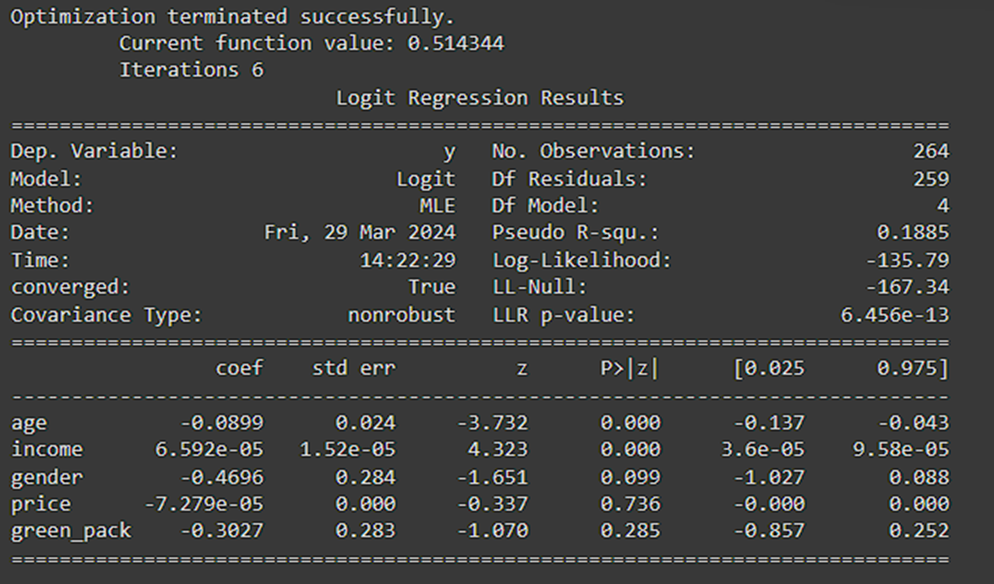
\includegraphics[height=6.6cm]{figures/coeff.png}
\caption{Parameters of the logistic regression model and their assessment}
\label{fig_regression}
\label{summary_lr}
\end{figure}

Figure \ref{summary_lr} shows the variables present in the data and their respective coefficients. It is evident that age and income are significant at 0.05 .We will now estimate the parameters of the logistic regression model, the values of which are given.

\begin{equation}
P(\text{Purchase} = \text{yes} | X) = \frac{e^{a}}{1 + e^{a}}
\label{LR_model}
\end{equation}
where
\begin{equation}
a = -0.0899 \times \text{age} + 6.592 \times 10^{-5} \times \text{income} - 0.4696 \times \text{gender} - 7.279 \times 10^{-5} \times \text{price} - 0.302 \times \text{green\_pack}
\label{LR_equation}
\end{equation}

Figure \ref{class_tab} shows the classification table. It can be seen that 66.67\% of the data is correctly classified. Only age and income are significant in explaining the decision of the consumer to purchase the product. The negative sign of the age coefficient indicates that older people generally don't buy products with green packaging and the positive coefficient of income shows that people with higher income mostly purchase the products with green packaging.


\begin{figure}[ht]
\centering
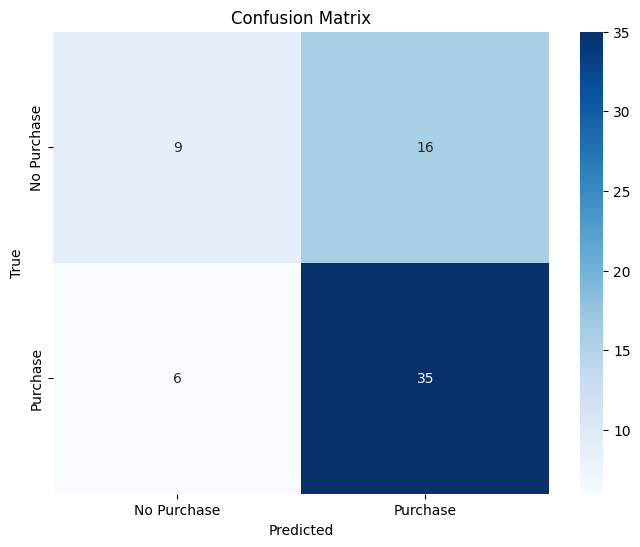
\includegraphics[height=6.6cm]{figures/confusion_matrix.png}
\caption{Classification Table}
\label{class_tab}
\end{figure}
\vspace{10pt}
Figure \ref{accuracy} shows the various accuracy measures to better understand the model


\begin{itemize}
    \item 	Precision: Precision measures the accuracy of positive predictions made by the model.
    \begin{equation}
        \text{Precision} = \frac{\text{True Positives}}{\text{True Positives} + \text{False Positives}}
    \end{equation}
    For class 0 (no purchase), it means that among the instances predicted as "no purchase" by the model, 60\% of them are actually "no purchase". Similarly, for class 1 (purchase), 69\% of instances predicted as "purchase" by the model are actually "purchase".
    \vspace{15pt}

    \item Recall/Sensitivity : Recall measures the ability of the model to correctly classify the positive instances.
       \begin{equation}
        \text{Sensitivity} = \frac{\text{True Positives}}{\text{True Positives} + \text{False Negatives}}
    \end{equation}
   The sensitivity of the model turns out to be 85\% which means that the model correctly identifies 85\% of the actual "purchase" instances.
    \vspace{15pt}

    \item Specificity : Specificity is an accuracy measure which represents the ability of the model to correctly classify the negatives instances. 
    \begin{equation}
        \text{Specificity} = \frac{\text{True Negatives}}{\text{True Negatives} + \text{False Positives}}

    \end{equation}
    
The specificity of the model is 36\% which means that for the "No purchases" class the model correctly identifies 36\% of the actual "no purchase" instances.
     \vspace{15pt}
 
    \item The F1-score is the harmonic mean of precision and recall. It provides a balance between precision and recall. For class 0 (no purchase), the F1-score is 0.45, and for class 1 (purchase), the F1-score is 0.76.

\end{itemize}

\begin{figure}[ht]
\centering
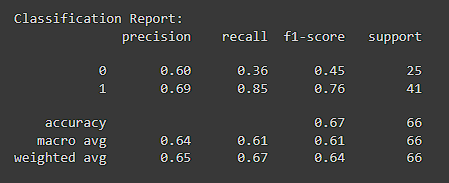
\includegraphics[height=4.5cm]{figures/accuracy.png}
\caption{Classification Report} 
\label{accuracy}
\end{figure}

\vspace{10pt}
\begin{figure}[ht]
\centering
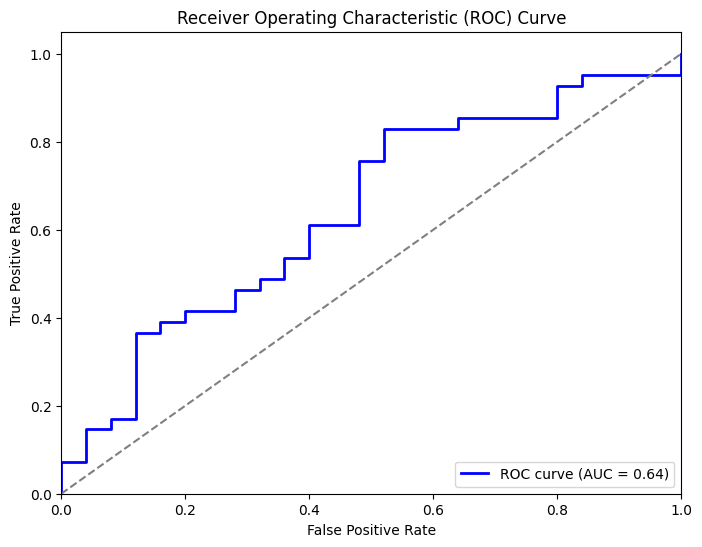
\includegraphics[height=6.6cm]{figures/AUC_ROC.png}
\caption{Receiver Operating Characteristic Curve} 
\label{auc}
\end{figure} 

\vspace{30pt}
Figure\ref{auc} shows the Receiver operating characteristic curve and the Area Under the curve of the model.
\begin{itemize}
    \item AUC is the proportion of the concordant pairs in the data if the model is used for classification. AUC for the data turned out to be \textit{0.64} which refers to \textbf{weak discrimination}. The model's performance is fair but there is room for improvement

    \item ROC curve can be used to understand the overall worth of the logistic regression model. Sensitivity is on the Y-axis and (1-Specificity) is on the X-axis. The straight line shows the 0.5 cut-off.
\end{itemize}


\section{Conclusion}
\begin{itemize}
    \item From the case it can be seen that the consumers belonging to an high income class are the ones who generally purchase products with green packaging. 
    \item Younger customers are more likely to purchase products with green packaging than older customers. 
    \item More awareness regarding green packaging should be spread in order to decrease and eventually eliminate non-recyclable waste.
\end{itemize}

\section{Future Scope}

As the data was stimulated for the purpose of understanding and applying logistic regression, the accuracy couldn't be high. More variables and real-life data can be taken into account to make more realistic and better prediction.



\fontsize{8}{9}\selectfont
\bibliography{ResearchPaperBib}



\clearpage



\end{document}